\documentclass[11pt]{article}
\usepackage[margin=1in]{geometry}
\usepackage{amsmath}
\usepackage{amssymb}
\usepackage{array}
\usepackage{booktabs}
\usepackage{float}
\usepackage{graphicx}
\usepackage{listings}
\usepackage{xcolor}
\usepackage[hidelinks]{hyperref}
\newcommand{\pra}{\mathrm{PRA}}
\newcommand{\refhandle}{\mathrm{REF}}
\newcommand{\kv}{\mathrm{KV}}
\newcommand{\q}{\mathbf{Q}}
\newcommand{\kmat}{\mathbf{K}}
\newcommand{\vmat}{\mathbf{V}}

\setlength{\emergencystretch}{3em}
\lstset{basicstyle=\ttfamily\footnotesize,breaklines=true,frame=single,columns=fullflexible}

\title{Oracle-First Native-K/V Materialization for Progressive Retrieval Attention:\\
Separating Memory Discovery from Physical Disclosure}
\author{Jorge Simao\\EInnovator R\&D -- Center for the Sciences of Computation, Cognition, and Complexity}
\date{\today}
\hypersetup{pdftitle={Oracle-First Native-K/V Materialization for PRA},pdfauthor={Jorge Simao}}

\begin{document}
\maketitle

\begin{abstract}
Sparse memory systems often treat finding a relevant region and loading its complete key/value
(K/V) payload as one operation.  This coupling obscures a separate question: once the relevant
conceptual memories are known, how much layer-native detail does a frozen transformer need?
We isolate that question in Progressive Retrieval Attention (PRA) by fixing dataset-annotated
evidence and varying only physical disclosure.  Materialization uses source-relative logical
intervals, unions overlap, crosses storage-chunk boundaries, preserves explicit-resource
boundaries and grouped-query-attention shapes, and transfers only gathered K/V from CPU to GPU.

Experiments use frozen Qwen3-0.6B on MuSiQue and 2WikiMultiHopQA.  Four validation examples per
dataset select a radius before an identity-disjoint eight-example held-out evaluation.  Exact
evidence disclosure preserves the same measured generated-answer F1 and normalized accuracy as
whole 32-token parent disclosure while reducing unique K/V by 19.8\% on MuSiQue and 53.0\% on
2Wiki.  The reduction is not free in likelihood: gold-token log probability falls by 0.246 and
0.210 nats/token, respectively, although evidence attention increases.  A 128-token cap is
97.5\% evidence-dense on MuSiQue but covers only 53.3\% of annotated evidence and degrades
likelihood; on 2Wiki it covers 96.6\% and nearly matches whole-parent likelihood.  In a separate
frozen Paper-2.5 selector factorial, local disclosure halves the graph-sparse payload on MuSiQue
and reduces it 38.2\% on 2Wiki; a 128-token cap raises 2Wiki output F1 from .50 to .75 but fails on
distributed MuSiQue evidence.  Native gist means do not substitute for token detail, and adding
them to local detail gives no consistent benefit.

The result is a bounded but useful claim.  Discovery breadth and active native K/V need not be
identical, and evidence-centered disclosure can reduce softmax competition and physical state.
Whether that reduction preserves model confidence depends on evidence distribution and memory-use
adaptation.  The study is a descriptive pilot, not a serving-speed or significance claim.
\end{abstract}

\section{Introduction}

A retrieval system answers at least three questions.  Which memory is relevant?  Which physical
detail should become active?  Can the model use that detail to produce the answer?  These questions
are easy to collapse because ordinary retrieval-augmented generation serializes selected text into
one prompt.  Once a document is selected, all of its re-tokenized prompt state participates in
attention.  Native-K/V memory exposes the separation more directly.  A compact representation can
identify a conceptual region while the attention kernel receives a smaller set of already computed
K/V states.

PRA Paper~1 separated logical memory from active attention state~\cite{simao2026pra}.  Paper~1.5
showed why semantic routing state and native positional attention state should remain distinct
\cite{simao2026position}.  Paper~2 integrated that boundary into pretrained Hugging Face decoder
families~\cite{simao2026hf}.  Paper~2.5 then treated discovery as bounded traversal over conceptual
memory regions.  The present paper asks the next question:
\begin{quote}
Once relevant conceptual memory is known, how little native K/V detail must be materialized for a
frozen model to preserve useful output behavior?
\end{quote}

The primary experiment begins with an oracle.  Dataset annotations specify the evidence intervals,
so a router cannot take credit or blame for the result.  We vary exact evidence, local context,
whole routing parents, fixed budgets, native gist means, and gist-plus-local hybrids.  Only after
freezing the oracle frontier do we cross Paper-2.5's one-shot and graph selectors with the same
materialization policies.  The experimental identity is therefore
\begin{equation}
 Q_{\mathrm{output}} = f(M\mid S),
\end{equation}
where selection $S$ is fixed within a comparison and materialization $M$ alone changes.

This distinction matters economically and scientifically.  Broad conceptual search can improve
recall, but whole-parent disclosure makes breadth expensive in K/V and introduces irrelevant
softmax competitors.  Conversely, a tiny physical budget can be evidence-dense while omitting
required evidence regions.  We therefore report both evidence density and evidence coverage,
rather than treating either as sufficient.

The contributions are:
\begin{enumerate}
\item a model-independent logical interval abstraction for layer-native K/V;
\item exact cross-chunk gathering with deduplication, resource isolation, GQA preservation, and
CPU-to-GPU transfer accounting;
\item an oracle-first M0--M7 materialization ladder and a predeclared radius/budget protocol;
\item paired output, attention, memory, and latency measurements on MuSiQue and 2Wiki;
\item a frozen selection-by-materialization factorial using Paper-2.5 conceptual selections; and
\item explicit negative results for native gist-only disclosure, hard-budget evidence truncation,
frozen MuSiQue memory use, and the absence of a serving-speed result.
\end{enumerate}

\section{Three Independent Decisions}

\subsection{Selection, materialization, and use}

Let $\mathcal{C}$ denote conceptual memory regions, $S(q,\mathcal{C})$ a selection procedure,
$M(S,B)$ a materializer under physical budget $B$, and $U$ the frozen transformer's native
attention and generation path.  PRA computes
\begin{align}
 C_q &= S(q,\mathcal{C}),\\
 (K_M,V_M) &= M(C_q,B),\\
 y &= U(q,K_M,V_M).
\end{align}
Paper~2.5 studies the first line.  This paper freezes the first line and studies the second.  A
memory-use adapter would change the third line and is outside the primary experiment.

This factorization prevents two misleading conclusions.  First, high evidence recall does not
prove that whole selected parents help output; their irrelevant K/V can dilute attention.  Second,
poor output after a small materialization does not prove that selection failed; the selected
concept may be correct while its disclosed detail lacks context.

\subsection{Three granularities}

We record three independent granularities:
\begin{equation}
 G_{\mathrm{encode}} \ne G_{\mathrm{search}} \ne G_{\mathrm{materialize}}.
\end{equation}
Canonical contextual K/V is encoded in model-safe blocks of 256 tokens.  Search addresses
32-token parents.  Materialization operates on arbitrary source-relative token intervals.  Storage
boundaries therefore do not define semantic windows.

\subsection{Logical materialization domains}

An interval is a half-open tuple
\begin{equation}
 I=(d,s,e),\qquad 0\le s<e,
\end{equation}
where $d$ is a logical domain.  Every explicit URI is a separate domain.  A window near the end of
one resource cannot continue into another resource merely because their tensors are adjacent in a
cache.  The displaced long-prompt resource \texttt{\#\_\_head} and the live prompt tail are one
exception: they share the continuous prompt-history domain established by canonical PRA.

For annotated evidence $[s_i,e_i)$, a symmetric local policy requests
\begin{equation}
 I_i(r)=[\max(0,s_i-r),\min(L_d,e_i+r)),
\end{equation}
with clipping inside domain $d$.  The physical request is the domain-wise union
\begin{equation}
 \mathcal{I}=\bigcup_i I_i,
\end{equation}
so each logical token is materialized at most once.

\section{Materialization Mechanism}

\subsection{Stored shards and canonical provenance}

Each reference layer stores shards with logical span, source URI, canonical post-position K/V, and
encoding provenance.  Primary experiments never re-encode isolated evidence.  If a semantic
window crosses two routing chunks, the gatherer slices both stored shards and concatenates them in
logical order.  For grouped-query attention, K/V remain
\begin{equation}
 [1,H_{kv},T,D_h],
\end{equation}
without expansion to query-head count.

Figure~\ref{fig:pipeline} shows the separation.  Conceptual selection stops before the physical
materializer.  The direct prompt K/V and selected memory K/V meet only at native attention.

\begin{figure}[H]
\centering
\fbox{\begin{minipage}{0.91\linewidth}
\centering
logical source / long prompt $\rightarrow$ model-safe contextual encoding blocks
$\rightarrow$ canonical native K/V shards\\[0.35em]
$\downarrow$\\[-0.25em]
smaller routing parents $\rightarrow$ gists / packed conceptual index
$\rightarrow$ fixed oracle or learned selection\\[0.35em]
$\downarrow$\\[-0.25em]
logical interval planner $\rightarrow$ domain union and deduplication
$\rightarrow$ cross-shard gather under K/V budget\\[0.35em]
$\downarrow$\\[-0.25em]
selected native K/V $+$ direct prompt K/V $\rightarrow$ pretrained native attention
\end{minipage}}
\caption{Selection and physical disclosure are separate operations.  Search parents are not
required to be encoding blocks or materialization windows.}
\label{fig:pipeline}
\end{figure}

\subsection{Cross-shard gather}

For each merged interval, the resolver advances a logical cursor.  Among overlapping storage
shards covering the cursor, it selects the shard extending furthest right, slices only the uncovered
range, and repeats until the interval ends.  Missing coverage raises an error instead of borrowing
tokens from another URI.  CPU-resident slices are collected before transfer; only the selected
slices move to the GPU.

\begin{lstlisting}[language=Python,caption={Simplified logical K/V gathering.}]
merged = union_intervals(requested_intervals)
for interval in merged:
    cursor = interval.start
    while cursor < interval.end:
        shard = furthest_shard_covering(interval.domain, cursor)
        stop = min(interval.end, shard.end)
        k_parts.append(shard.k[:, :, cursor-shard.start:stop-shard.start, :])
        v_parts.append(shard.v[:, :, cursor-shard.start:stop-shard.start, :])
        cursor = stop
K = torch.cat([part.to(device) for part in k_parts], dim=2)
V = torch.cat([part.to(device) for part in v_parts], dim=2)
\end{lstlisting}

The implementation records requested tokens before union, deduplicated tokens, materialized bytes,
evidence and non-evidence tokens, shards touched, cross-shard interval count, interval-resolution
time, gather time, and host-to-device time.

\subsection{Fixed budgets across evidence regions}

For $n$ regions with capacities $c_i$, a fixed budget assigns integer quotas $b_i$ satisfying
\begin{equation}
 1\le b_i\le c_i,\qquad \sum_i b_i\le B.
\end{equation}
Equal, evidence-length-proportional, minimum-core-plus-remainder, and score-proportional allocation
are implemented.  Gate~1 uses equal allocation.  Every region receives at least one token, but a
budget smaller than the complete evidence cores may explicitly truncate those cores.  Evidence
coverage exposes that truncation; it is never inferred from density.

\section{Oracle Policy Ladder}

Table~\ref{tab:policies} defines the non-learned ladder.  M4 is not a separate tensor path:
deduplication is mandatory for every interval policy.  M6 first forms radius-64 candidates and then
allocates the fixed physical budget.

\begin{table}[H]
\centering
\caption{Oracle-first disclosure policies.}
\label{tab:policies}
\small
\begin{tabular}{p{0.09\linewidth}p{0.28\linewidth}p{0.53\linewidth}}
\toprule
Policy & Name & Physical disclosure \\
\midrule
M0 & native gist only & One native-head mean K/V state per selected parent \\
M1 & whole parent & Every K/V token in each selected 32-token routing parent \\
M2 & evidence only & Exact union of annotated evidence token intervals \\
M3 & local window & Symmetric radii $r\in\{0,4,8,16,32,64\}$ \\
M4 & deduplicated windows & Domain-wise union before physical gather; active in M2--M7 \\
M5 & asymmetric window & Eight tokens left and 32 tokens right of evidence \\
M6 & fixed budget & Equal allocation at 64, 128, and 256 native K/V tokens \\
M7 & gist plus local & Native K/V mean for every selected parent plus local token K/V \\
\bottomrule
\end{tabular}
\end{table}

The native gist in M0/M7 is deliberately not the routing vector.  On a GQA model, routing width can
equal hidden size while native K/V width is $H_{kv}D_h$.  We instead average each parent's actual
native K and V independently over tokens, preserving the physical head layout.

\section{Experimental Protocol}

\subsection{Model, data, and frozen controls}

Table~\ref{tab:protocol} summarizes the experiment.  MuSiQue and 2Wiki retain their annotation
graphs and exact serialized source spans from Paper~2.5.  Validation and held-out identities are
disjoint.  No optimization occurs in this paper.

\begin{table}[H]
\centering
\caption{Frozen oracle-frontier protocol.}
\label{tab:protocol}
\small
\begin{tabular}{p{0.30\linewidth}p{0.59\linewidth}}
\toprule
Property & Value \\
\midrule
Backbone & Qwen3-0.6B, frozen, eager native attention, FP16 CUDA \\
Datasets & MuSiQue and 2WikiMultiHopQA annotated development examples \\
Selection & Dataset evidence oracle for Gate~1; frozen Paper-2.5 selectors for Gate~2 \\
Validation / held-out & 4 / 8 identity-disjoint examples per dataset \\
Selector factorial & 4 held-out examples per dataset, 4 selectors $\times$ 4 policies \\
$G_{encode}/G_{search}$ & 256 / 32 source tokens \\
Materialization layers & Inherited Paper-2.5 bands: all 28 for MuSiQue; layers 12,20,24,27 for 2Wiki \\
Direct prompt / native limit & 128 / 4096 tokens \\
Decode & Greedy, at most 12 new tokens; brief-answer extraction \\
Validation rule & Smallest radius within 0.05 nats/token of whole-parent likelihood; otherwise best likelihood \\
Hardware & NVIDIA GeForce GTX 950M, 4 GB; reference K/V resident on CPU \\
\bottomrule
\end{tabular}
\end{table}

The validation rule selects radius zero on both datasets.  Held-out evaluation therefore compares
M2 evidence only without revisiting the radius choice.  We report exact match, token F1, containment,
normalized answer accuracy, gold answer log probability, attention mass, K/V tokens and bytes,
evidence density and coverage, peak CUDA memory, TTFT, TPOT, and gather/transfer timing.

The optional dense full-context control exceeded the 4~GB GPU during eager attention and is omitted.
This does not remove the whole-parent PRA ceiling, but it prevents a direct full-context comparison.
Timing is synchronized single-example research timing; it is not a loaded-serving benchmark.

\section{Oracle Frontier Results}

\subsection{Validation selects exact evidence}

Figure~\ref{fig:frontier} shows the validation frontier.  Increasing radius does not monotonically
improve likelihood.  Exact evidence is the strongest measured point on both validation slices.
On MuSiQue it uses 350.5 rather than 415.5 unique K/V tokens and improves likelihood from
$-9.073$ to $-8.281$.  On 2Wiki it uses 82.8 rather than 144.0 tokens and improves likelihood from
$-4.716$ to $-4.354$.  These four-example values select the policy; they are not the final estimate.

\begin{figure}[H]
\centering

\includegraphics[width=0.98\linewidth]{../shared/results/paper3_kv_materialization/oracle_materialization_frontier.pdf}
\caption{Validation quality/K/V frontier, quality versus radius, and evidence density.  Radius zero
is selected before held-out evaluation.}
\label{fig:frontier}
\end{figure}

\subsection{Held-out quality and K/V}

Table~\ref{tab:heldout} gives the held-out result.  Exact evidence preserves the same generated
answer metrics as whole parents on both datasets.  This is useful but should not be overstated:
MuSiQue F1 is zero for both policies, while 2Wiki F1 and normalized accuracy are .50.  Likelihood
detects a cost hidden by those coarse output metrics.

\begin{table}[H]
\centering
\caption{Held-out oracle disclosure, eight examples per dataset.  LP is mean gold-token log
probability.  Coverage is fraction of annotated evidence physically present.}
\label{tab:heldout}
\small
\begin{tabular}{llrrrrrr}
\toprule
Dataset & Policy & K/V & Reduction & Density & Coverage & LP & F1 \\
\midrule
MuSiQue & whole parent & 313.5 & 0.0\% & .802 & 1.000 & $-8.774$ & .000 \\
MuSiQue & evidence only & 253.1 & 19.8\% & 1.000 & 1.000 & $-9.020$ & .000 \\
MuSiQue & budget 128 & 128.0 & 57.2\% & .975 & .533 & $-9.542$ & .000 \\
\midrule
2Wiki & whole parent & 136.0 & 0.0\% & .470 & 1.000 & $-5.528$ & .500 \\
2Wiki & evidence only & 62.5 & 53.0\% & 1.000 & 1.000 & $-5.738$ & .500 \\
2Wiki & budget 128 & 124.9 & $-6.7$\% & .476 & .966 & $-5.551$ & .500 \\
\bottomrule
\end{tabular}
\end{table}

Evidence-only likelihood falls 0.246 nats/token on MuSiQue and 0.210 on 2Wiki relative to whole
parents.  It wins or ties on three of eight and two of eight paired examples, respectively.  The
result supports K/V compression at fixed deterministic output, not likelihood equivalence.

\subsection{Attention dilution}

The smaller disclosure concentrates attention.  Evidence attention rises from .522 to .662 on
MuSiQue and from .161 to .194 on 2Wiki.  Thus less irrelevant K/V produces more evidence-directed
attention, even when likelihood does not improve.  This separates a mechanistic effect from an
output claim: removing softmax competitors is measurable, but the frozen model may still need
surrounding context or adaptation to interpret the remaining states.

\begin{figure}[H]
\centering
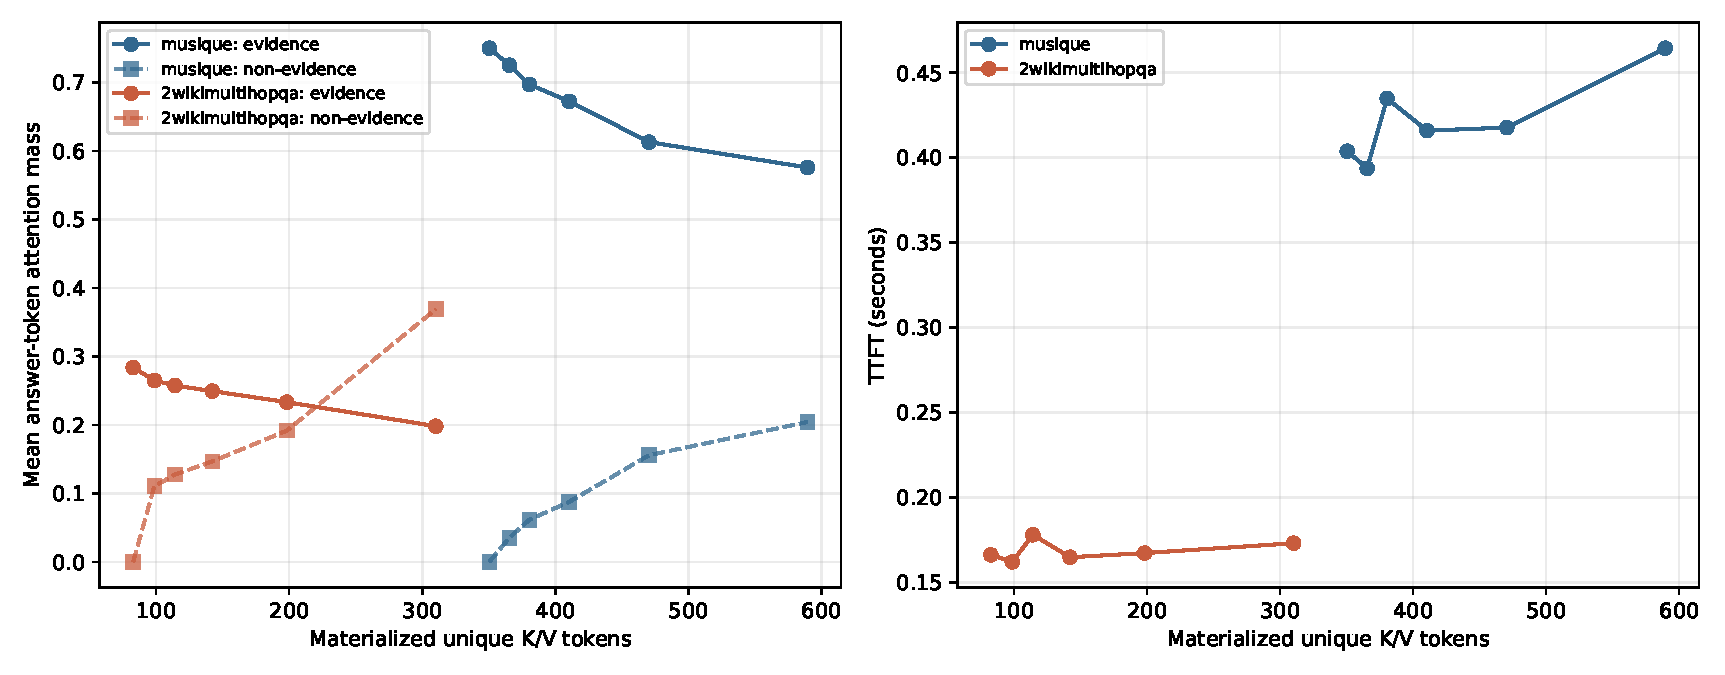
\includegraphics[width=0.94\linewidth]{../shared/results/paper3_kv_materialization/materialization_dilution_latency.pdf}
\caption{Validation evidence/non-evidence attention and synchronized TTFT against materialized K/V.
The small pilot does not support a serving-speed claim.}
\label{fig:dilution}
\end{figure}

\subsection{Density is not coverage}

The fixed-budget result is the clearest warning.  MuSiQue budget-128 disclosure is 97.5\%
evidence-dense, apparently an efficient payload, but it includes only 53.3\% of the annotated
evidence core.  Its likelihood loses another 0.522 nats/token relative to exact evidence.  On
2Wiki, the same policy covers 96.6\% of evidence and is only 0.023 nats/token below whole parents.
The parameter is identical; evidence distribution differs.

This result rejects a simple global rule such as ``128 K/V tokens are enough.''  A fixed budget
needs evidence-region-aware feasibility or an adaptive stopping criterion.  Minimum one-token
allocation prevents silent total starvation, but it cannot preserve a long evidence paragraph.

\subsection{Gists are routing state, not sufficient detail}

M0 reduces K/V by about 97\%, but MuSiQue likelihood is 7.374 nats/token below whole parents and
2Wiki is 0.582 below.  M7 adds one native gist per selected parent to exact evidence.  It changes
MuSiQue likelihood by less than .001 relative to evidence only and loses .007 on 2Wiki, while using
more K/V.  Mean native K/V therefore does not replace token detail in this configuration and does
not justify a hybrid default.

\subsection{Frozen memory-use boundary}

No-memory likelihood is $-4.491$ on held-out MuSiQue, substantially above every memory policy.
On 2Wiki, whole-parent memory improves over no memory by 0.564 nats/token and evidence-only improves
by 0.354.  Paper~3 does not solve this dataset-level consumption mismatch because the backbone and
memory-use path are frozen.  The MuSiQue result is evidence against interpreting an oracle K/V
frontier as proof that a pretrained model can use all annotated evidence.  The materializer can be
correct while the consumer is not calibrated.

\section{Frozen Selection by Materialization}

After Gate~1, we reuse one-shot, graph-sparse, graph-balanced, and graph-high Paper-2.5 selected
spans.  Oracle annotations are unavailable to both selection and interval construction.  For each
selector we compare the selected 32-token parents, the selector's own atomic logical spans, a
128-token equal allocation, and native gist plus atomic detail.

\begin{table}[H]
\centering
\caption{Representative selector/materializer pairs, four held-out examples per dataset.  $\Delta$
LP and $\Delta$F1 are relative to the same selector with whole-parent disclosure.}
\label{tab:factorial}
\small
\begin{tabular}{llrrrrr}
\toprule
Dataset & Selector / disclosure & Parents & K/V & Reduction & $\Delta$LP & $\Delta$F1 \\
\midrule
MuSiQue & graph sparse / local & 13.75 & 216.2 & 49.4\% & $-0.153$ & .000 \\
MuSiQue & graph sparse / budget 128 & 13.75 & 128.0 & 69.8\% & $-6.690$ & .000 \\
MuSiQue & graph balanced / budget 128 & 11.75 & 128.0 & 91.4\% & $-8.273$ & .000 \\
\midrule
2Wiki & graph sparse / local & 14.00 & 221.5 & 38.2\% & $+0.069$ & $+.250$ \\
2Wiki & graph sparse / budget 128 & 14.00 & 128.0 & 63.3\% & $+0.223$ & $+.250$ \\
2Wiki & graph balanced / budget 128 & 6.00 & 128.0 & 81.8\% & $+0.280$ & $+.250$ \\
2Wiki & graph high / budget 128 & 9.50 & 128.0 & 87.8\% & $+0.427$ & $+.250$ \\
\bottomrule
\end{tabular}
\end{table}

Graph-sparse selection supplies the cleanest direct test because its selected atomic spans are
finer than their storage parents.  Local materialization nearly halves MuSiQue payload with a
modest likelihood loss and reduces 2Wiki payload while improving both likelihood and F1.  For
one-shot, graph-balanced, and graph-high conditions, many selected spans already cover complete
32-token parents or merge into broad contiguous regions, so local materialization is identical to
whole-parent disclosure.  Multi-scale discovery does not guarantee a finer physical payload if
its final selected intervals are coarse.

The hard budget again exposes a dataset interaction.  Every reported 2Wiki selector reaches F1
.75 under 128 tokens, compared with .50 for its whole-parent counterpart.  MuSiQue remains at the
zero-F1 floor and suffers large likelihood losses.  Smart materialization can bound broad
conceptual discovery on 2Wiki, but a common global budget does not yet handle MuSiQue's distributed
multi-region evidence.

\begin{figure}[H]
\centering
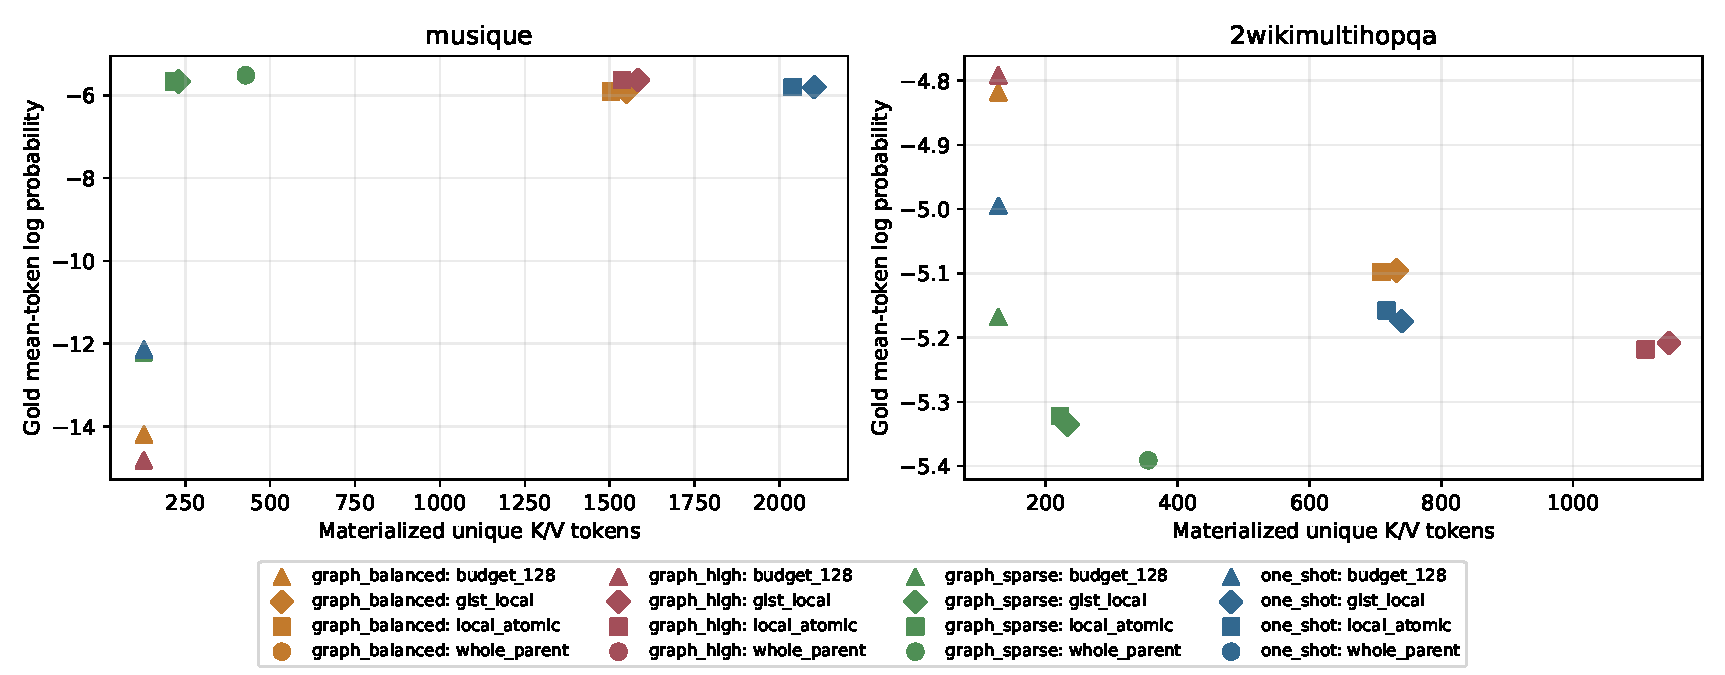
\includegraphics[width=0.92\linewidth]{../shared/results/paper3_kv_materialization/selector_materialization_factorial.pdf}
\caption{Frozen selection-by-materialization factorial.  The same conceptual selection can occupy
different physical K/V points; broad selected spans sometimes leave no local compression room.}
\label{fig:factorial}
\end{figure}

\begin{figure}[H]
\centering
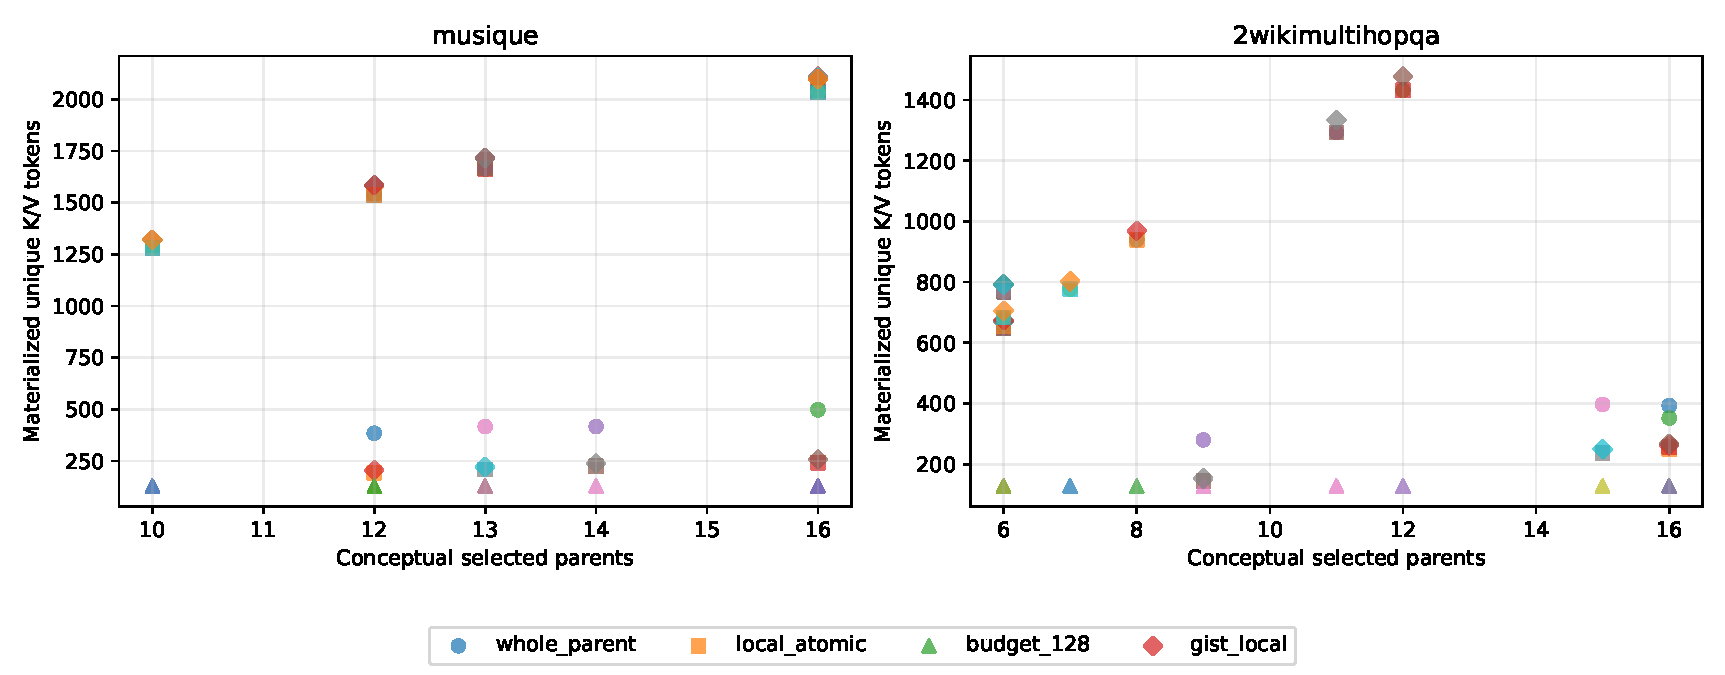
\includegraphics[width=0.92\linewidth]{../shared/results/paper3_kv_materialization/conceptual_breadth_physical_kv.pdf}
\caption{Conceptual parent count versus physical K/V.  Fixed budgets decouple the axes, but quality
depends on whether the budget preserves all required evidence regions.}
\label{fig:breadth}
\end{figure}

\section{Systems Accounting}

Reference K/V remains on CPU in native KV-head form.  The materializer slices CPU tensors before
transfer and records final H2D bytes/time.  On the held-out oracle evidence condition, summed
cross-shard interval counts are 63 per MuSiQue example across 28 active layers and 7 per 2Wiki
example across four active layers.  Thus semantic evidence commonly crosses storage boundaries;
clipping at the selected parent would change the experiment.

Deduplication also has observable effect.  Held-out 2Wiki evidence requests average 65.1 tokens
before union and materialize 62.5, a 4.0\% reduction.  Validation radius 64 requests 338.8 and
materializes 310.3, an 8.4\% reduction.  MuSiQue's selected examples contain little interval
overlap, so deduplication saves little there.  Deduplication is semantically required even when it
does not dominate runtime.

TTFT does not monotonically follow selected K/V in this small synchronized experiment.  Evidence
only is 0.080 seconds slower than whole parents on MuSiQue and 0.008 seconds slower on 2Wiki.
Python interval resolution, many small slices, eager attention, Windows WDDM, and single-example
noise dominate the token reduction.  The result is a memory frontier, not a speed frontier.  Fused
interval indexing and batched gathers belong to a systems follow-up.

\section{Implementation and Reproducibility}

The implementation is split at the same conceptual boundaries as the method.  In the revision
used for this paper:
\begin{itemize}
\item \texttt{src/pra\_torch/materialization.py:35} defines logical intervals;
\item line 81 defines provenance-bearing K/V shards;
\item line 225 performs domain-wise interval union;
\item line 312 allocates fixed budgets across regions;
\item lines 378--401 resolve exact cross-shard coverage; and
\item line 403 gathers ordered K/V and records physical/transfer metrics.
\end{itemize}

The shared execution core parses interval requests at
\texttt{src/pra\_torch/core.py:211}, materializes them at line 249, constructs native gist controls
at line 359, and dispatches all legacy and Paper-3 disclosure modes through the same fixed-selection
boundary at line 449.  The public and internal HF configurations expose
\texttt{detail\_materialization}; reference construction records encoding granularity in
\texttt{src/pra\_torch/hf/injection.py:446}.

The oracle harness, selector factorial, and analysis are in
\path{experiments/paper3_kv_materialization}.  Canonical JSON/CSV rows and figures are under
\path{docs/papers/shared/results/paper3_kv_materialization}.  Each experiment writes a JSONL
checkpoint after every condition.  Dataset annotations enter Gate~1 interval planning but are
explicitly unavailable to Gate~2 selectors and materializers.

\section{Related Work}

Sparse-attention architectures reduce the token pairs processed inside a model through fixed or
learned patterns~\cite{beltagy2020longformer}.  Recurrent and compressed-context approaches retain
history through cache policies or summary state; StreamingLLM studies stable attention sinks for
streaming caches~\cite{xiao2023streamingllm}, while Infini-attention introduces compressive memory
inside attention~\cite{munkhdalai2024infini}.  Memorizing Transformers retrieve approximate
nearest-neighbor K/V from prior examples~\cite{wu2022memorizing}, and landmark attention separates
block-level addressing from token-level access~\cite{mohtashami2023landmark}.  These systems differ
in training and storage contracts, but they motivate separating compact addressing from detailed
state.

PRA's materialization question is narrower.  The selected payload is layer-native contextual K/V,
the host backbone is frozen, and the experiment begins with oracle evidence so retrieval recall
cannot confound disclosure.  The contribution is not a new end-to-end long-context benchmark
leader.  It is a controlled physical interface and evidence about how output changes along its
K/V frontier.

\section{Limitations}

The held-out oracle study has eight examples per dataset and the selector factorial has four.
Results are descriptive; no confidence interval or significance claim is warranted.  Greedy exact
match and F1 are coarse, particularly on MuSiQue where every compared condition is at the zero-F1
floor.  A validated blinded LLM judge has not yet been run for Paper~3.

Only Qwen3-0.6B is evaluated.  Materialization behavior may differ with model scale, family,
fine-tuning, quantization, and attention kernel.  The inherited all-28 MuSiQue materialization band
is expensive and may amplify frozen-model interference.  We preserve it to avoid selecting a new
layer policy on the materialization outcome.

The evidence oracle assumes dataset annotations identify useful source spans.  It does not prove
that every token in an annotated paragraph is causally necessary.  Conversely, exact evidence can
lack discourse or entity context outside the annotation.  M2's likelihood loss is consistent with
that possibility but does not identify the cause by itself.

The direct full-context control OOMed on the available 4~GB GPU under dense eager attention.
Latency uses a single Windows GPU without loaded concurrency, and Python gather overhead remains.
The paper therefore makes no production throughput, cost, or asymptotic speed claim.

\section{Discussion and Paper-3.5 Handoff}

The central hypothesis survives in a qualified form.  Conceptual discovery breadth and physical
native K/V can be decoupled.  Exact evidence often occupies substantially less K/V than whole
routing parents, increases evidence attention, and preserves the measured greedy answer metrics.
The likelihood penalty shows that annotations alone do not specify all useful context.  A practical
materializer should therefore choose context adaptively rather than assume either whole parents or
zero radius.

Three next steps follow directly.  First, budget allocation should preserve complete evidence cores
before distributing remainder, or explicitly defer a region rather than truncate it.  Second,
selected native positions should seed asymmetric windows whose size depends on boundary,
punctuation, and confidence.  Third, materialization and memory-use adaptation should be trained
jointly only after retaining the oracle controls; otherwise an adapter can conceal disclosure
failure.

Paper~3.5 receives a concrete interface: logical intervals, cross-shard gather, exact metrics,
radius-zero and 128-token target points, CPU/GPU transfer profiles, and the observed gather
bottleneck.  It should own learned adaptive budgets, fused indexing/gather kernels, batching,
concurrency, and cross-family serving measurements.

\section{Conclusion}

Finding memory and loading memory are different operations.  Under oracle selection, exact
evidence reduces active native K/V and softmax competition while preserving the measured generated
answer scores, but it does not preserve gold-token likelihood exactly.  Fixed budgets work when
they retain the evidence distribution and fail when density hides low coverage.  With frozen
Paper-2.5 selectors, sparse conceptual discovery benefits most from finer disclosure; broad
selected spans may leave nothing to compress.  These results establish materialization as its own
research object and provide a reproducible boundary for the next systems and learning stage.

\appendix

\section{Test Matrix}

Focused tests cover intervals inside one shard, one-boundary and multi-boundary gathers, overlapping
storage shards, overlapping requested intervals, exact token order, resource start/end clipping,
explicit-resource rejection, \texttt{\#\_\_head}-to-prompt continuity, GQA shape preservation,
CPU-to-GPU transfer bytes, fixed budgets, multi-evidence allocation, radius zero, whole-parent
equivalence, logical-core metrics, native gist controls, and budget rejection.  Existing PRA,
Paper-2, and Paper-2.5 regressions run in the full project suite.

\section{Canonical Row Schema}

Every result row records dataset and identity, selection and materialization policy, radii and K/V
budget, conceptual parents, intervals, requested and deduplicated tokens, unique tokens, per-layer
token states and bytes, evidence/non-evidence tokens, density and coverage, layer band, output and
teacher-forced metrics, attention mass, interval/gather/H2D timing, TTFT, TPOT, total generation,
throughput, and peak CUDA allocated/reserved bytes.  Oracle use is an explicit boolean.

\section{Negative Result Ledger}

\begin{table}[H]
\centering
\small
\begin{tabular}{p{0.29\linewidth}p{0.62\linewidth}}
\toprule
Observation & Consequence \\
\midrule
Native gist-only collapses quality & Gists remain routing/index state, not a default detail payload. \\
Evidence-only loses likelihood & Zero-radius evidence is a compression point, not universal equivalence. \\
MuSiQue budget 128 covers 53.3\% & Density must always be paired with evidence coverage. \\
Frozen MuSiQue replay loses to no memory & Correct materialization does not solve memory-use calibration. \\
Broad selected spans do not shrink locally & Finer physical disclosure requires finer selected intervals or a within-parent policy. \\
Python gather does not improve TTFT & Optimize indexed/fused gather before speed or cost claims. \\
Direct full context OOMs & No dense full-context ceiling is reported on the 4~GB device. \\
No blinded judge yet & Behavioral equivalence is limited to deterministic and teacher-forced metrics. \\
\bottomrule
\end{tabular}
\end{table}

\bibliographystyle{plain}
\bibliography{../shared/references}

\end{document}
